\begin{figure}
	\centering
	\pgfplotsset{every axis legend/.append style={
		at={(1.05,0.5)},
		anchor=west}}
	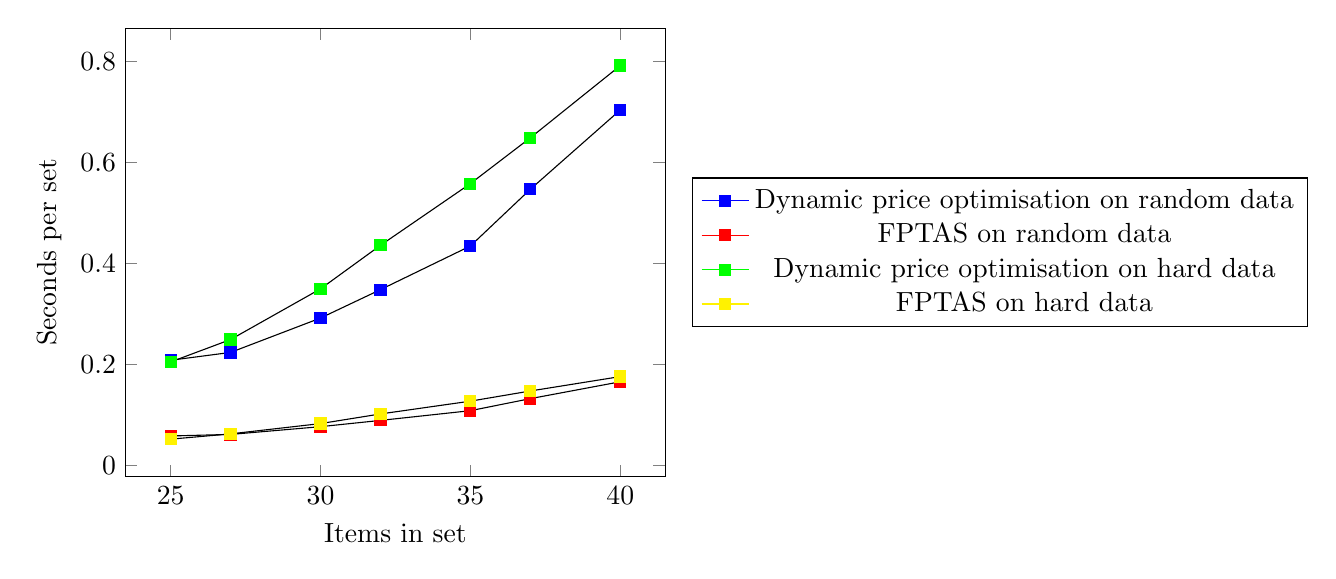
\begin{tikzpicture}
		\begin{axis}[
			xlabel=Items in set,
			ylabel=Seconds per set,
			scatter/classes={
				dynN={mark=square*,blue},
				fptasN={mark=square*,red},
				dynH={mark=square*,green},
				fptasH={mark=square*,yellow}
				}
			]
			\addplot[scatter,%
				scatter src=explicit symbolic]%
			table[meta=label] {
				x y label
				25 .208052 dynN
				27 .223608 dynN
				30 .291732 dynN
				32 .348044 dynN
				35 .434604 dynN
				37 .547092 dynN
				40 .704324 dynN
			};
			\addplot[scatter,%
				scatter src=explicit symbolic]%
			table[meta=label] {
				x y label
				25 .057974 fptasN
				27 .061048 fptasN
				30 .076414 fptasN
				32 .088828 fptasN
				35 .108118 fptasN
				37 .132000 fptasN
				40 .165394 fptasN
			};
			\addplot[scatter,%
				scatter src=explicit symbolic]%
			table[meta=label] {
				x y label
				25 .204710 dynH
				27 .249138 dynH
				30 .349580 dynH
				32 .435896 dynH
				35 .558234 dynH
				37 .649110 dynH
				40 .792216 dynH
			};
			\addplot[scatter,%
				scatter src=explicit symbolic]%
			table[meta=label] {
				x y label
				25 .051640 fptasH
				27 .062136 fptasH
				30 .082542 fptasH
				32 .101642 fptasH
				35 .126996 fptasH
				37 .147170 fptasH
				40 .175732 fptasH
			};
			\addlegendentry{Dynamic price optimisation on random data}
			\addlegendentry{FPTAS on random data}
			\addlegendentry{Dynamic price optimisation on hard data}
			\addlegendentry{FPTAS on hard data}
		\end{axis}
	\end{tikzpicture}
\caption{Time needed depending on number of items in set (closer look)}
\label{plot:cutTime}
\end{figure}
